\speciestitle{Bromine monoxide}{BrO}{BrO}{%
\item[Useful range: ] 10--3.2\,hPa (day/night differences needed)
\item[Contact:] Luis Mill\'an, \email{Luis.F.Millan@jpl.nasa.gov}}
\subsection{Introduction}

The standard product for BrO is taken from the 640-GHz \texttt{CoreR4AB14}
retrieval. The spectral signature of BrO in the MLS radiances is very
small, leading to a very poor signal-to-noise ratio on individual MLS
observations.  Significant averaging (e.g., monthly zonal means) is
required to obtain scientifically useful results.  Large biases of
between 12 to 43\,pptv (typical BrO abundances range from 5 to 15\,pptv)
are seen in the data. These biases can be minimized by taking day/night
differences. For pressures of 4.6 hPa and greater, nighttime BrO is
negligible; however, for smaller pressures, nighttime BrO needs to be
taken into account. Table~\ref{tab:BrOSummary} summarizes the precision,
accuracy, and resolution of the MLS \thisv\CheckThis BrO product. The accuracy
assessment is based on v2.2 data, as described in the validation paper
\citep{KovalenkoEtal:2007:BrO}.

Note, the \thisv\CheckThis ``standard'' BrO product (as with earlier versions)
contains systematic biases and horizontal oscillations that present a
larger challenge than for other species.  Those interested in using
MLS BrO in scientific studies are strongly advised to contact the MLS
team before embarking on their research.  Different algorithms for BrO
have been developed by the MLS team, aimed at ameliorating some of
these artifacts \citep{MillanEtal:2012}, and those products are
available from the GSFC DISC\@.  The product short name is
``\texttt{ML3DZMBRO}'' and it is available from:
\url{https://disc.gsfc.nasa.gov/datacollection/ML3DZMBRO_004.html}.

\subsection{Vertical Resolution}
\oneverticalavk{BrO}{BrO}

Figure~\ref{fig:AvkBrO} shows that the vertical resolution for the \thisv\CheckThis
MLS BrO is about 5.5\,km in the 10 to 4.6\,hPa pressure region, 
degrading to 6\,km at 3.2\,hPa.

\subsection{Precision}

\begin{figure}
\begin{center}
  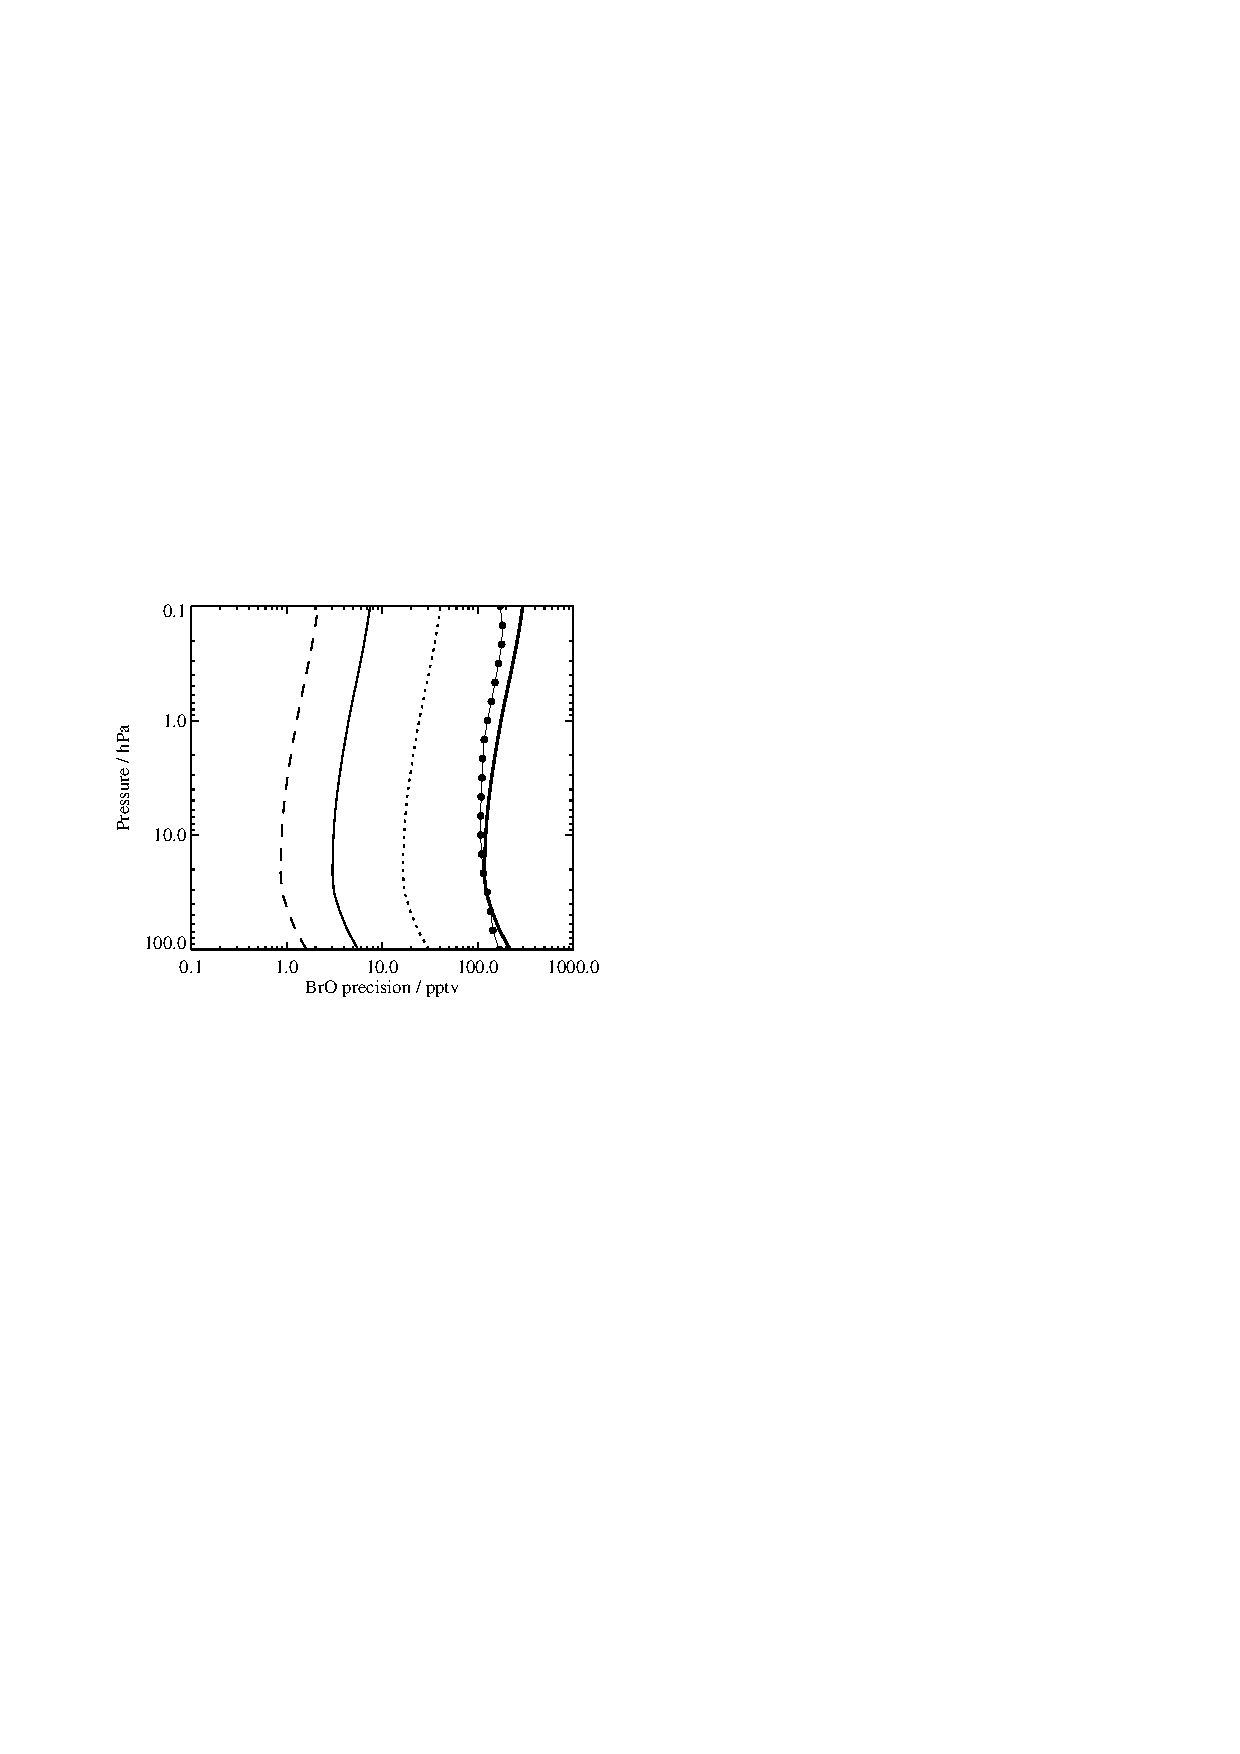
\includegraphics[width=0.4\linewidth]{figures/bro-precision}
\end{center}
\caption{Comparison of the MLS \thisv\CheckThis BrO precision as estimated from
  scatter in the retrieved data (circles) with that expected from the
  retrieval (thick line), for a single profile.  Also shown is the
  expected precision for the day/night difference of 10\degsym\ zonal
  mean profiles averaged over a day (dotted line), a month (thin line)
  and a year (dashed line).}
\label{fig:BrOPrecision}
\end{figure}

The expected precision in a retrieved profile is calculated from
radiance noise and reported for each retrieved data point.  The value of
the expected precision is flagged negative or zero if it is worse than
50\% of the value of the a priori precision.
Figure~\ref{fig:BrOPrecision} compares the expected precision (thick
line) on an individual MLS BrO measurement with that deduced from
observations of scatter in night-time observations (expected to be
zero). Also shown are the expected precisions for daily, monthly, and
yearly 10\degsym\ zonal means. For the minimal averaging recommended, a
monthly 10\degsym\ zonal mean, which corresponds to about 3,000
measurements, the precision is about $\pm$4\,ppt. See
Table~\ref{tab:BrOSummary} for more details.

\subsection{Accuracy}

The accuracy of the MLS BrO product is summarized in
Table~\ref{tab:BrOSummary}. The effect of each identified source of
systematic error on MLS measurements of radiance has been quantified and
modeled \citep{ReadEtal:2007}. These quantified effects correspond to
either $2\sigma$ estimates of uncertainties in each MLS product, or an
estimate of the maximum reasonable uncertainty based on instrument
knowledge and/or design requirements. More discussion is given in
\cite{KovalenkoEtal:2007:BrO}.  While that paper described v2.2 BrO, findings
are expected to be applicable also to \thisv\CheckThis. The potential systematic
bias in MLS BrO measurements can be as high as about $\pm$43\,ppt at
10\,hPa, decreasing to about $\pm$12\,pptv at 3.2\,hPa. The systematic
bias is dramatically reduced by subtracting the nighttime signal from
the daytime signal.  Taking the day/night difference reduces the
systematic biases to $\pm$16\,pptv at 10\,hPa and to $\pm$9\,pptv at
3.2\,hPa.  If the MLS BrO data is used at 3.2 hPa, the day/night
difference value will need to be adjusted to compensate for the
non-negligible nighttime BrO. We note that this method of taking
day/night differences is not applicable for polar summer and winter
during periods of continuous sunlight or darkness.

\subsection{Data screening}
\label{sec:BrOScreening}
\begin{description}
\item[Pressure range:] \screeningrule{10--3.2 hPa} \standardrangestatement
\item[Averaging required:] \screeningrule{Significant averaging (such as
    monthly zonal means) is required if useful scientific data are
    sought.}
\item[Diurnal differences:] \screeningrule{For use in any scientific
    study, day / night or ascending / descending differences should be used
    to alleviate biases.}  Note that, for 3.2\,hPa, the non-zero
  nighttime expected abundances BrO needs to be taken into account.
  \standardprecisionrule \evenstatusrule
\item[Clouds:] \cloudsokrule
\item[Quality:] \qualityrule{1.3}
\item[Convergence:] \convergencerule{1.05}
\end{description}

\subsection{Artifacts}
Significant biases exist in the BrO data, as discussed above. Day /
night (or ascending / descending) differences must be used to reduce
these.  For 3.2 hPa, nighttime BrO needs to be taken into account
\citep{KovalenkoEtal:2007:BrO}.

A systematic horizontal (i.e., profile-to-profile) oscillation has been
discovered in MLS \thisv\CheckThis (and earlier) standard BrO product.  This
presents a significant challenge to the interpretation of the BrO
observations.  Users are strongly advised to contact the MLS team before
embarking on research involving the MLS standard BrO product.  As
described above, use of other BrO products is preferable to using the
Level~2 BrO data.

\subsection{Review of comparisons with other data sets}
We have calculated total bromine, Br$_{y}$, from MLS measurements of BrO
using a photochemical model, and compared this with Br$_{y}$ similarly
inferred from balloon-borne measurements of BrO; good agreement is seen
\citep{KovalenkoEtal:2007:BrO}.


\begin{table}
\caption{Summary of the Aura MLS \thisv\CheckThis BrO product.}
% \caption{Summary of the Aura MLS BrO product.}
\vspace{\tablecaptionsep}
\label{tab:BrOSummary}
\begin{minipage}{\linewidth}
\centering\begin{tabular}{ccccl}
\toprule
\parbox[m]{5em}{\bfseries\centering Pressure range} &
\parbox[m]{4em}{\bfseries\centering Vertical res. / km} &
\parbox[m]{5.0em}{\bfseries\centering Precision\footnote{The precision quoted is for a 10\degsym\
    monthly zonal mean} / pptv} &
\parbox[m]{5.0em}{\bfseries\centering Day/night difference accuracy\footnote{Because of large biases in
    the data, the daytime and nighttime BrO data are unsuitable for
    scientific use, so day/night differences must be used. Note that
    day/night differences are not useful for polar winter and summer,
     where BrO does not undergo a diurnal variation.} / pptv} &
\textbf{Comments} \\
\midrule
%
2.2\,hPa and less & -- & -- & -- & Unsuitable for scientific use
  \\ %\addlinespace[2ex]
%
3.2\,hPa & 6 & $\pm$5 &$\pm$8
& \parbox[m]{10em}{\raggedright Need to
account for non-negligible night time BrO} \\ \addlinespace[2ex]

%
4.6 & 5.5 & $\pm$4 & $\pm$10  \\
6.8 & 5.5 & $\pm$4 & $\pm$11 \\ 
10  & 5.5 & $\pm$4 & $\pm$13 \\ 
150--15\,hPa   & -- & -- & -- & Unsuitable for scientific use \\
1000--215\,hPa & -- & -- & -- & Not retrieved \\
\bottomrule
\end{tabular}
\end{minipage}
\end{table}







%%% Local Variables: 
%%% mode: latex
%%% TeX-master: "v5-x-report"
%%% End: 
